\documentclass{article}

\usepackage{hyperref}

% Below will configure hyperlink colors
\hypersetup{
    colorlinks=true,
    linkcolor=blue,
    filecolor=blue,
    urlcolor=blue,
}
\urlstyle{same}

\usepackage{enumitem}

% Below package is for precise positioning of images
\usepackage{float}
\usepackage{color}

% Below package is for syntax highlighted code
\usepackage{minted}
% Below set global setting fro minted package like line wraps and frame
\setminted{breaklines, frame=single}

% Below package is for including images
\usepackage{graphicx}
\usepackage[a4paper, inner=1.5cm, outer=3cm, top=2cm,bottom=3cm, bindingoffset=1cm]{geometry}
\setlength{\parskip}{.5em}

% The LaTeX graphics/graphicx package uses the first dot to find the extension. Package grffile changes this algorithm. This helps in including images files whose name contains more than 1 dot
\usepackage{grffile}


% Below package will create headings
%\pagestyle{headings}

% Below package will used to specify captions like "Figure 1: Nice Figure" in minipages using \captionof{figure}{Nice Figure}
\usepackage{caption}
\usepackage{hypcap} %This is needed for some warning in minipages


\begin{document}
\begin{titlepage}
   \vspace*{\stretch{1.0}}
   \begin{center}
      \Large\textsc{PCI Express Basics 101}\\
      \vspace{5mm}
      \Large\textit{Vineel Kovvuri}\\
      \url{http://vineelkovvuri.com}\\
   \end{center}
   \vspace*{\stretch{2.0}}
\end{titlepage}

\tableofcontents

\newpage
\section{Introduction}
PCI Express: It is a standard which comes in multiple generations
and multiple lane configurations. PCI-E is in its 5th generation,
but mostly the current shipping generation is 3rd generation also
called as Gen 3. Mainly each generation improves upon the previous
generation regarding the speed per lane supported by the protocol.

Below is the table for each generation and lane speed 
For single-lane (×1) and 16-lane (×16) links, in each direction:
\begin{center}
\begin{tabular}{|c|c|c|}
 Generation &x1         &x16          \\
 \hline
 Gen 1      &250 MB/s   &4 GB/s       \\
 Gen 2      &500 MB/s   &8 GB/s       \\
 Gen 3      &985 MB/s   &15.75 GB/s   \\
 Gen 4      &1.969 GB/s &31.51 GB/s   \\
 Gen 5      &3.938 GB/s &63 GB/s
\end{tabular}
\end{center}

There are PCIE connectors in x1, x2, x4, x8, x16 configurations.
The specification also makes sure in an x16 physical connector
we can plugin in any card with x1, x2, x4, x8, x16. One important fact
about physical connectors is, x16 physical may not be powering
all the 16 lanes so for example in a motherboard if an x16 connector
is fueling only x4 lanes, it means, The connector is limited to x4 speeds.

\begin{figure}[H]
\centering
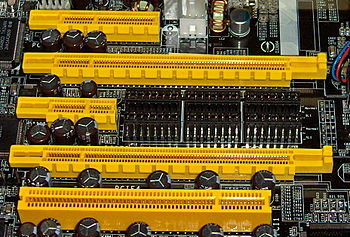
\includegraphics[width=\textwidth]{350px-PCIExpress.png}
\caption{Different type of physical PCIE connectors}
\end{figure}

Now to understand each connectors capability we need to refer the
motherboard manual. They explicitly talk about the supported
connectors and their configuration for the CPU maximum
supported lane count. After all CPU max supported PCI-E lane count
is what matters and how the motherboard takes advantage of these lanes.

\begin{figure}[H]
\centering
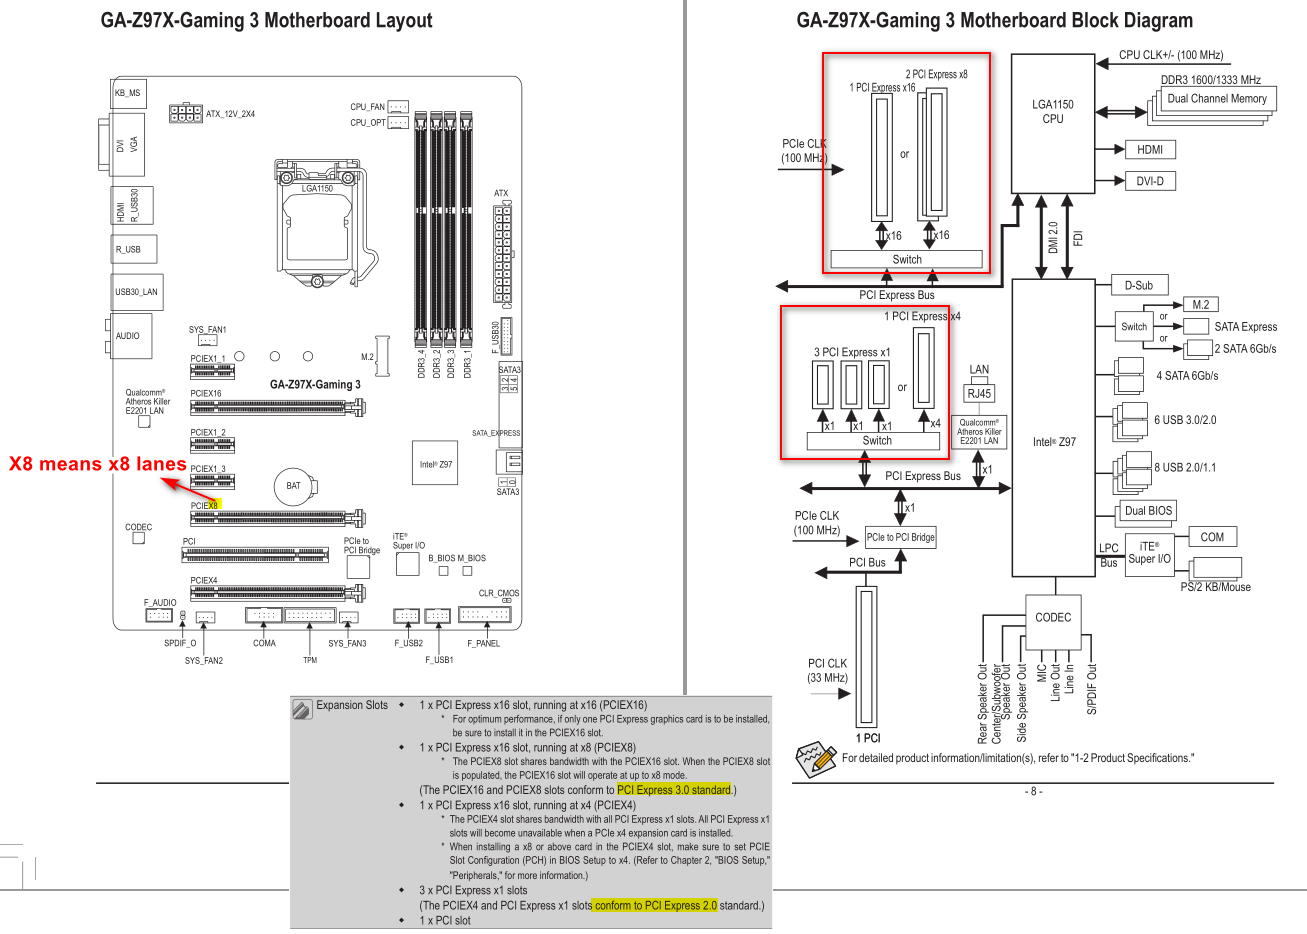
\includegraphics[width=\textwidth]{Motherboard-Manual.png}
\caption{Gigabyte Motherboard manual description of on board PCIE connectors and their configurations}
\end{figure}


\section{References}
\begin{enumerate}[noitemsep]
\item \href{https://computer.howstuffworks.com/pci-express.htm}{How PCI Express Works}
\end{enumerate}



\end{document}